\chapter{Showtime}\label{chap:Showtime}

The showtime is the final part of the master project where all groups are presenting their projects and their results.
Before the showtime was beginning a lot of planning was necessary. From the actual presentation and equipment to the brochures and posters. Everything needed to be planned and organized.

\section{Paperwork}
At the beginning it was necessary to make a first concept of the brochure and posters for the unplagged exhibition stand.

\pagebreak

\subsection{Brochure}
The first concept of the brochure was kind of a sketch.

\begin{figure}[!h]
  \centering
  \fbox{
    
\includegraphics[width=0.97\textwidth]{images/brochure_sketch.png}
  }
  \caption{the first concept of the brochure}
  \label{fig:brochure_sketch}
\end{figure}
\pagebreak
Below is the final outlook of the brochure.

\begin{figure}[!h]
  \centering
  \fbox{
    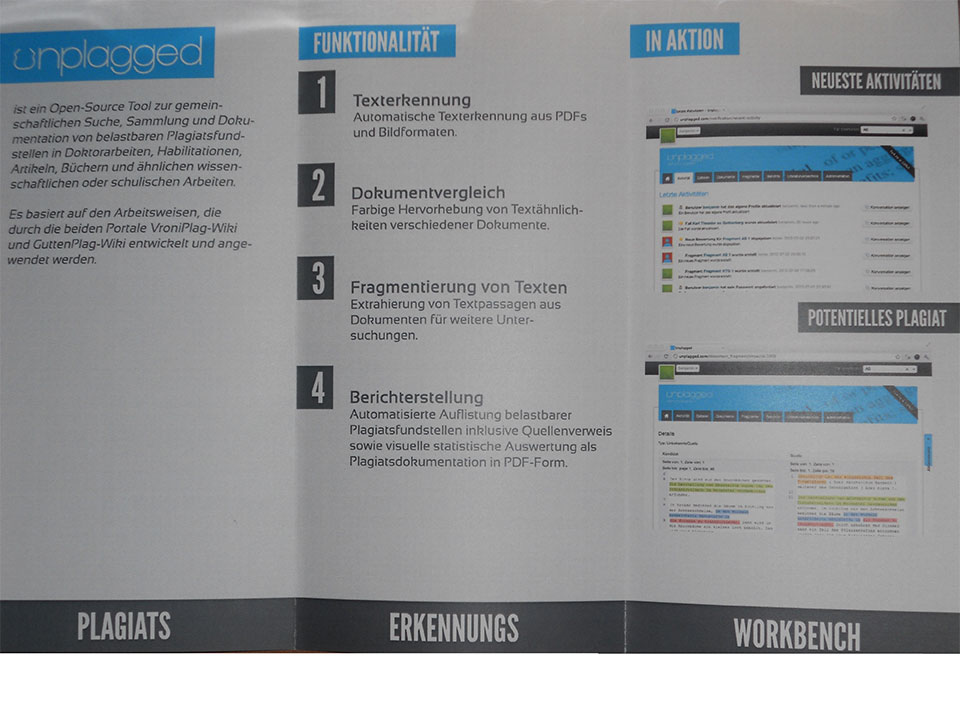
\includegraphics[width=0.97\textwidth]{images/brochure_final_frontside.jpg}
  }
  \caption{the frontside of the final unplagged brochure}
  \label{fig:brochure_final_frontside}
\end{figure}

\begin{figure}[!h]
  \centering
  \fbox{
    
\includegraphics[width=0.97\textwidth]{images/brochure_final_backside.jpg}
  }
  \caption{the backside of the final unplagged brochure}
  \label{fig:brochure_final_backside}
\end{figure}

\pagebreak 

\subsection{Posters}

\subsubsection{Title Poster}
The title poster shows the name of the unplagged master project.

\begin{figure}[!h]
  \centering
  \fbox{
    
\includegraphics[width=0.97\textwidth]{images/poster_title.jpg}
  }
  \caption{the title poster}
  \label{fig:poster_title}
\end{figure}

\pagebreak

\subsubsection{Describing Poster}

Here it is the outlook of the poster which has short describings about the project.

\begin{figure}[!h]
  \centering
  \fbox{
    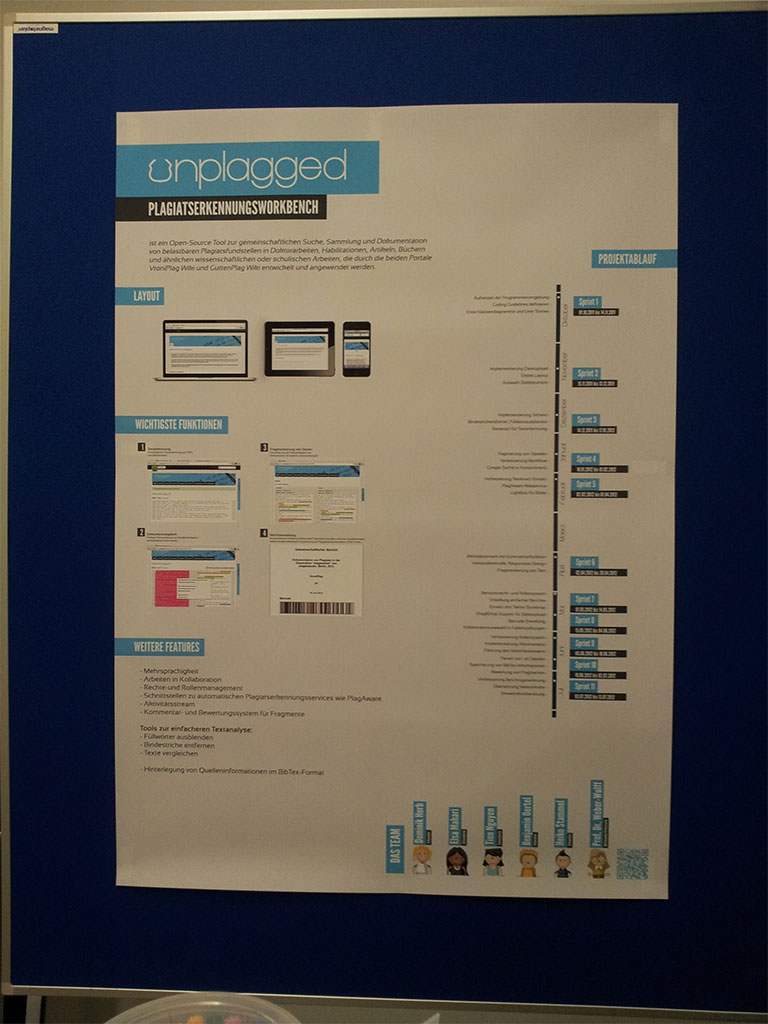
\includegraphics[width=0.97\textwidth]{images/poster_describing.jpg}
  }
  \caption{the describing poster}
  \label{fig:poster_describing}
\end{figure}

\pagebreak

\subsubsection{Technical Poster}

Below is a cutout of the technical poster.

\begin{figure}[!h]
  \centering
  \fbox{
    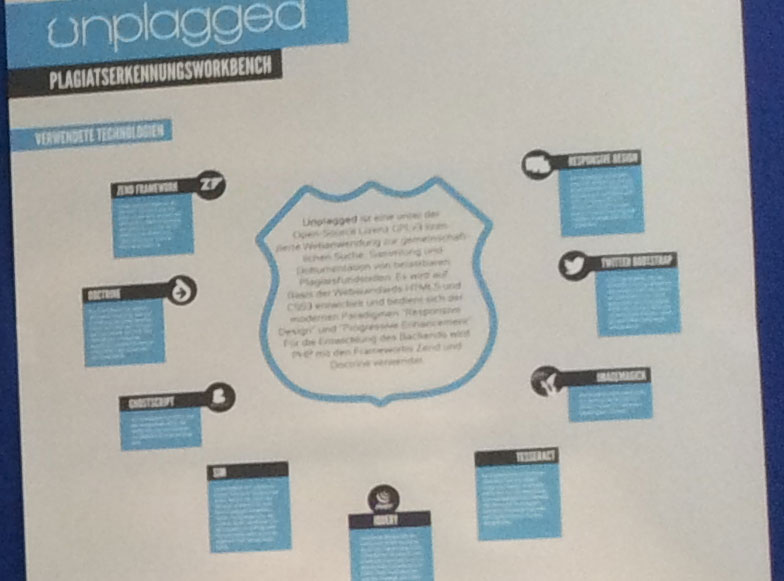
\includegraphics[width=0.97\textwidth]{images/poster_technical.jpg}
  }
  \caption{the technical poster}
  \label{fig:poster_technical}
\end{figure}

\pagebreak 

\section{Equipment}
Below there is the list of the equipment which was used for the unplagged exhibition stand.

\begin{itemize}
\item 3 iMacs
\item 3 tables
\item 2 higher tables
\item 3 pinboards
\item 2 floodlights
\end{itemize}

\pagebreak 

\section{Outlook of the exhibition stand}
Below there are some snapshots of the unplagged exhibition stand.


\begin{figure}[!h]
  \centering
  \fbox{
    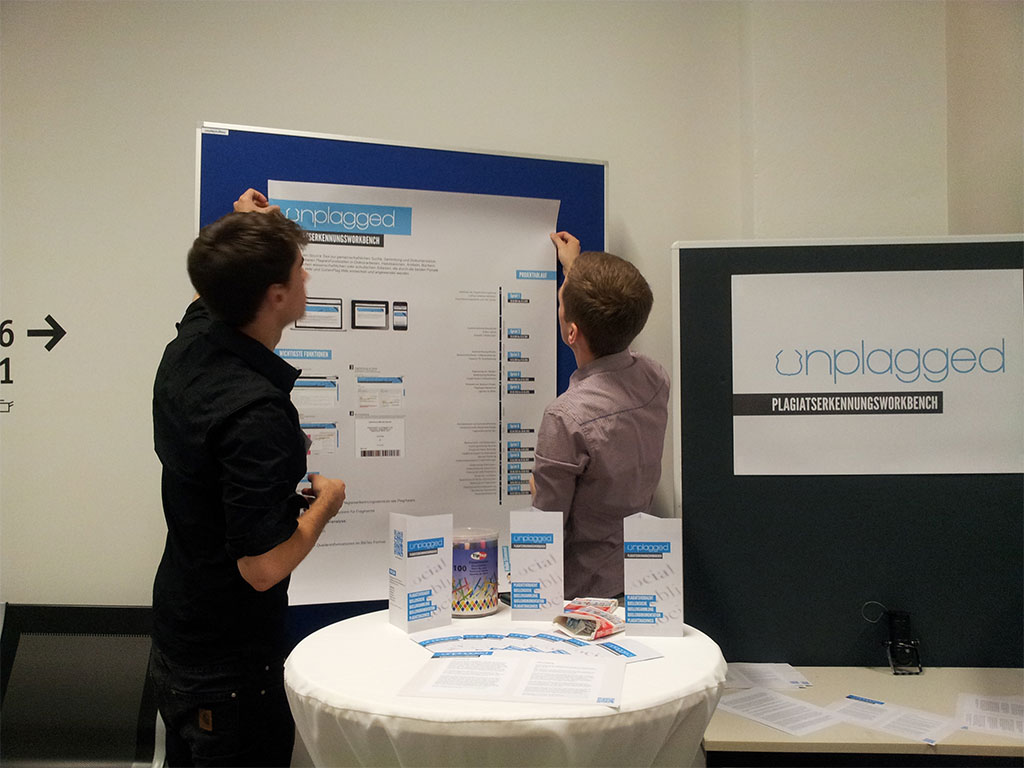
\includegraphics[width=0.97\textwidth]{images/unplagged_exhibition_stand1.jpg}
  }
  \caption{unplagged exhibition stand}
  \label{fig:unplagged_exhibition_stand1}
\end{figure}

\pagebreak

\begin{figure}[!h]
  \centering
  \fbox{
    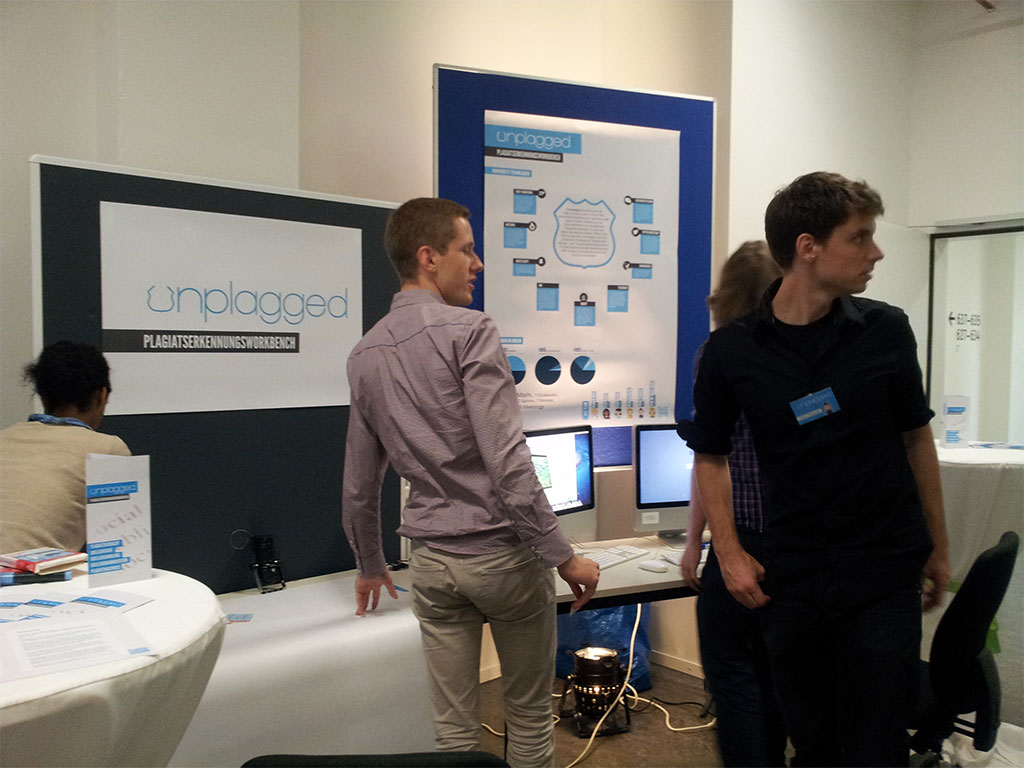
\includegraphics[width=0.97\textwidth]{images/unplagged_exhibition_stand2.jpg}
  }
  \caption{unplagged exhibition stand}
  \label{fig:unplagged_exhibition_stand2}
\end{figure}

\pagebreak 

\begin{figure}[!h]
  \centering
  \fbox{
    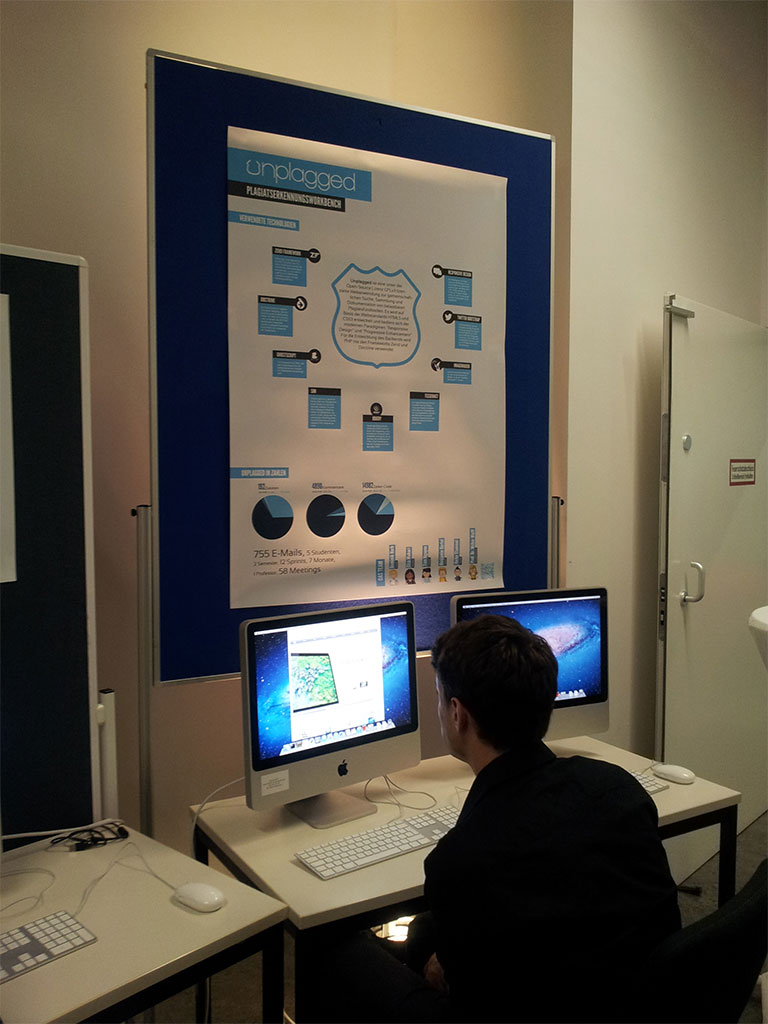
\includegraphics[width=0.97\textwidth]{images/unplagged_exhibition_stand3.jpg}
  }
  \caption{unplagged exhibition stand}
  \label{fig:unplagged_exhibition_stand3}
\end{figure}

\pagebreak

\begin{figure}[!h]
  \centering
  \fbox{
    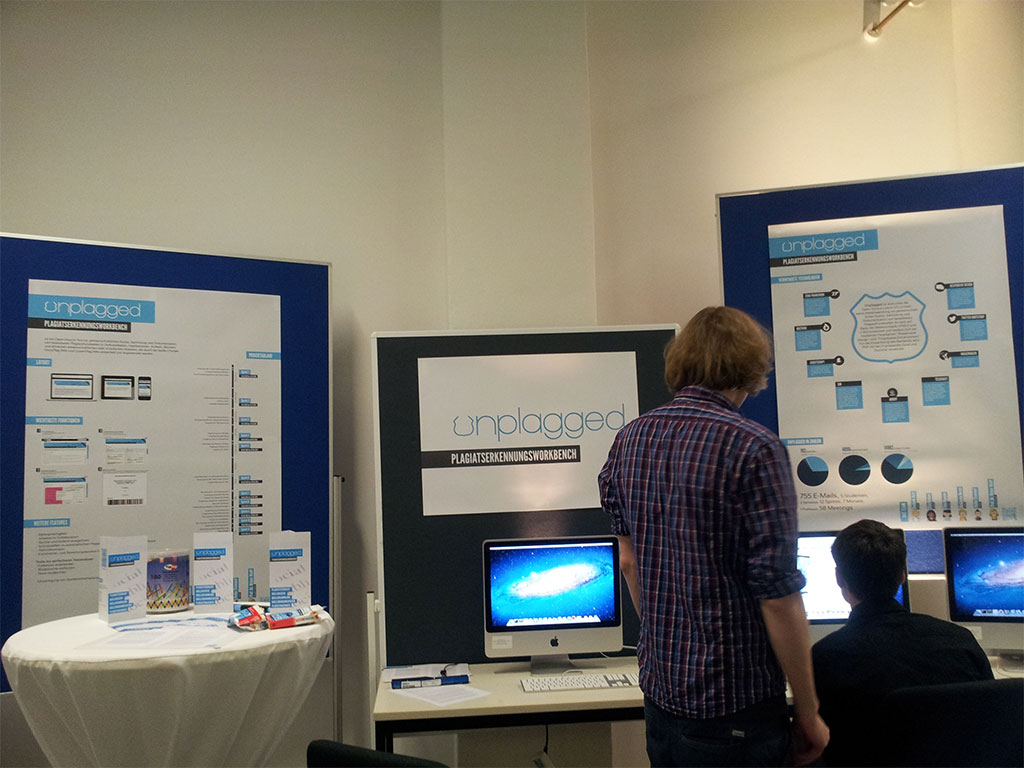
\includegraphics[width=0.97\textwidth]{images/unplagged_exhibition_stand4.jpg}
  }
  \caption{unplagged exhibition stand}
  \label{fig:unplagged_exhibition_stand4}
\end{figure}

\pagebreak